\section{Desarrollo del sistema.}

En esta sección vamos a dar paso al desarrollo del proyecto, en primer lugar hablaremos sobre la implementación de la red
blockchain en las Raspberry previamente configuradas, para pasar al desarrollo de la API basada en GraphQL con NodeJS y 
posteriormente a la interfaz de usuario con Gatsby y React.  

\subsection{Configuración y creación de la topología de la red.}

\begin{figure}[ht!]
  \centering
  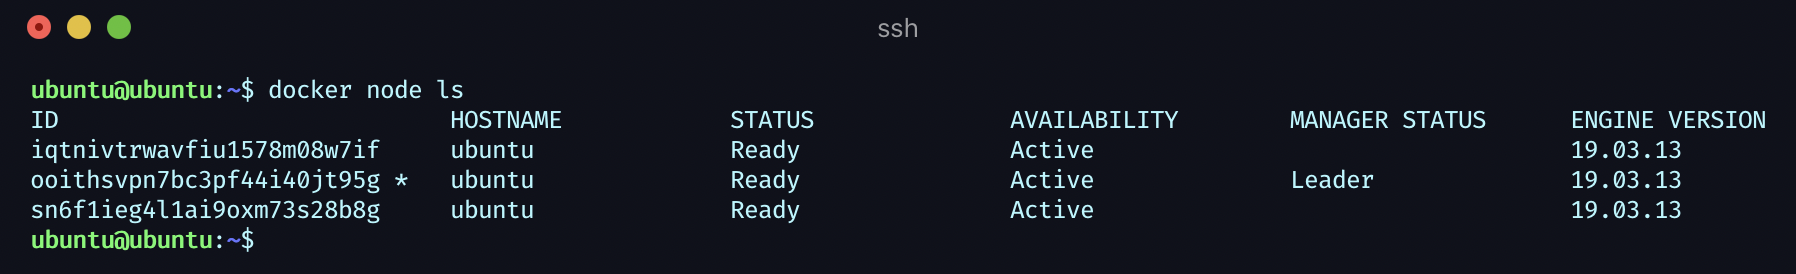
\includegraphics[width=10cm]{imagenes/desarrollo/comandos/node_ls_worker}
  \caption{Nodos de Docker Swarm.}
  \label{fig:node-ls-worker}
\end{figure}

\begin{figure}[ht!]
  \centering
  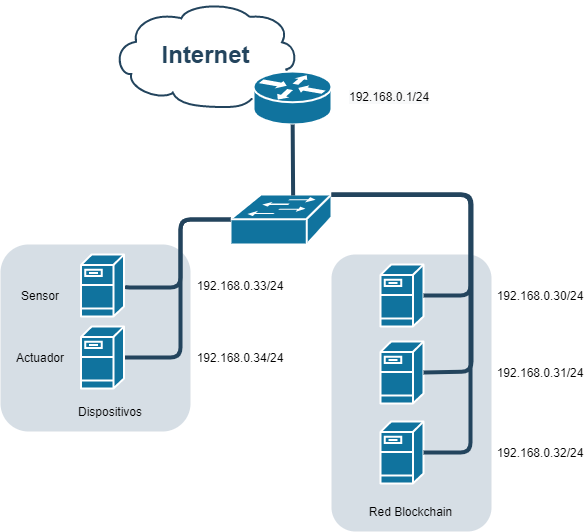
\includegraphics[width=10cm]{imagenes/desarrollo/topologia_red}
  \caption{Topología de la red.}
  \label{fig:topologia-red}
\end{figure}

\begin{figure}[ht!]
  \centering
  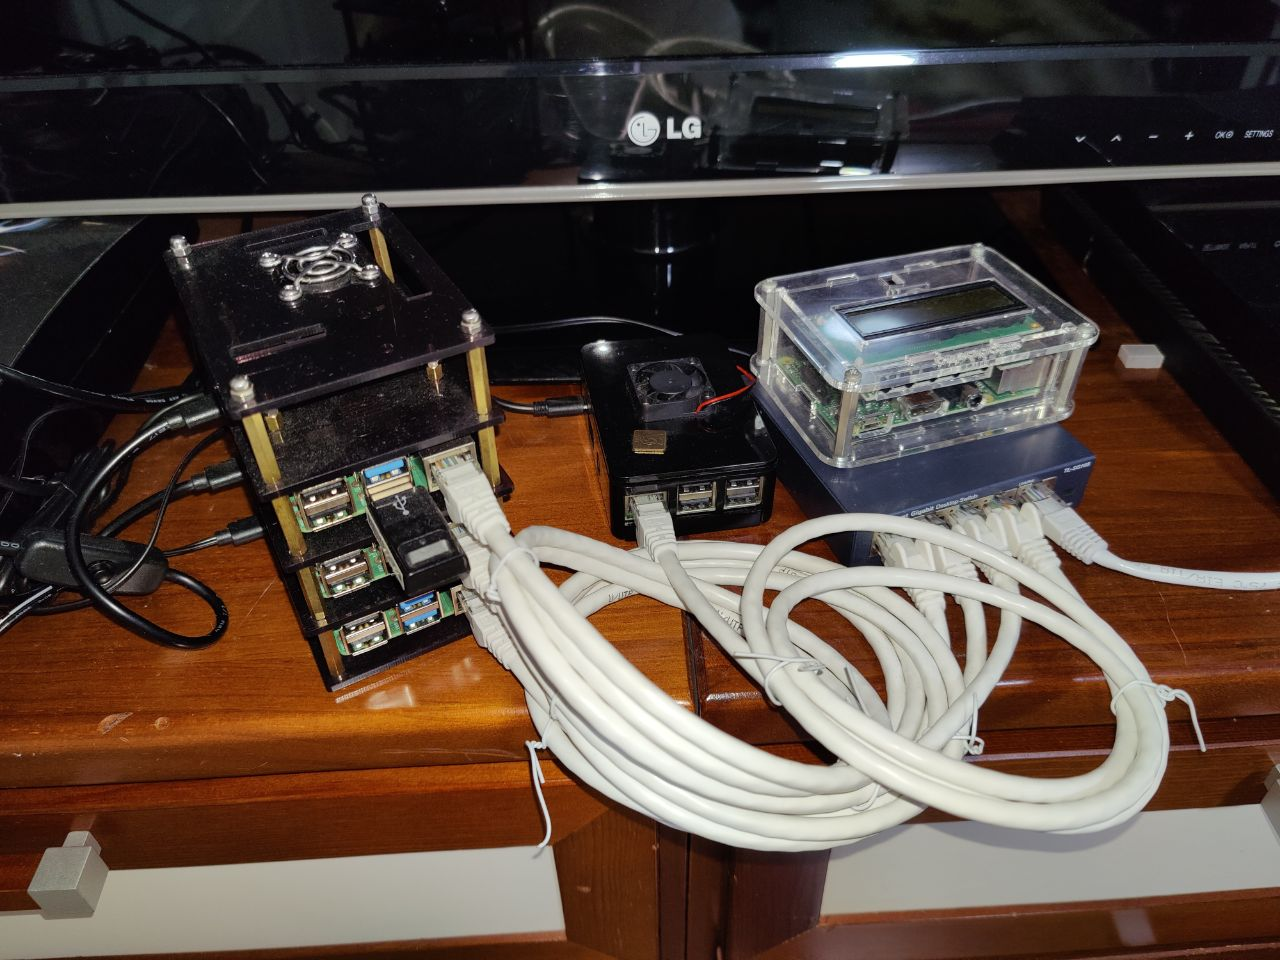
\includegraphics[width=10cm]{imagenes/desarrollo/foto_raspberry}
  \caption{Captura de las Raspberry Pi.}
  \label{fig:captura-raspberry}
\end{figure}

\begin{figure}[ht!]
  \centering
  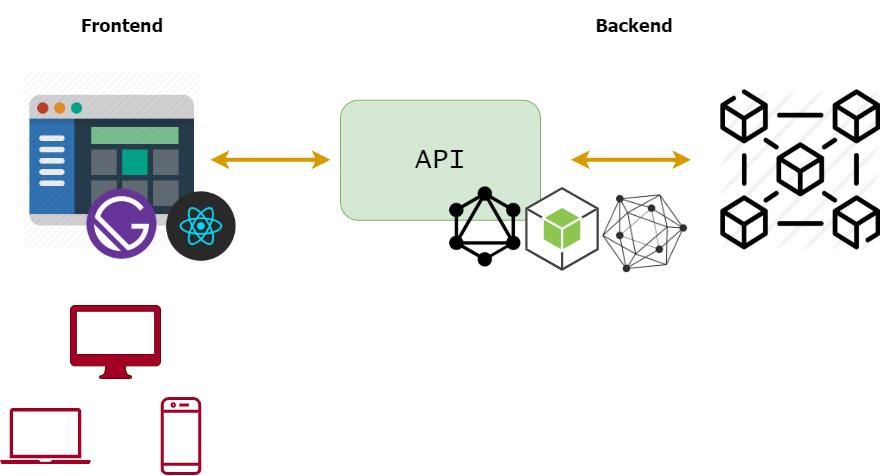
\includegraphics[width=10cm]{imagenes/desarrollo/arquitectura_aplicacion}
  \caption{Arquitectura de la aplicación.}
  \label{fig:arquitectura-aplicacion}
\end{figure}

\subsection{Implementación de la red Blockchain.}

\begin{figure}[ht!]
  \centering
  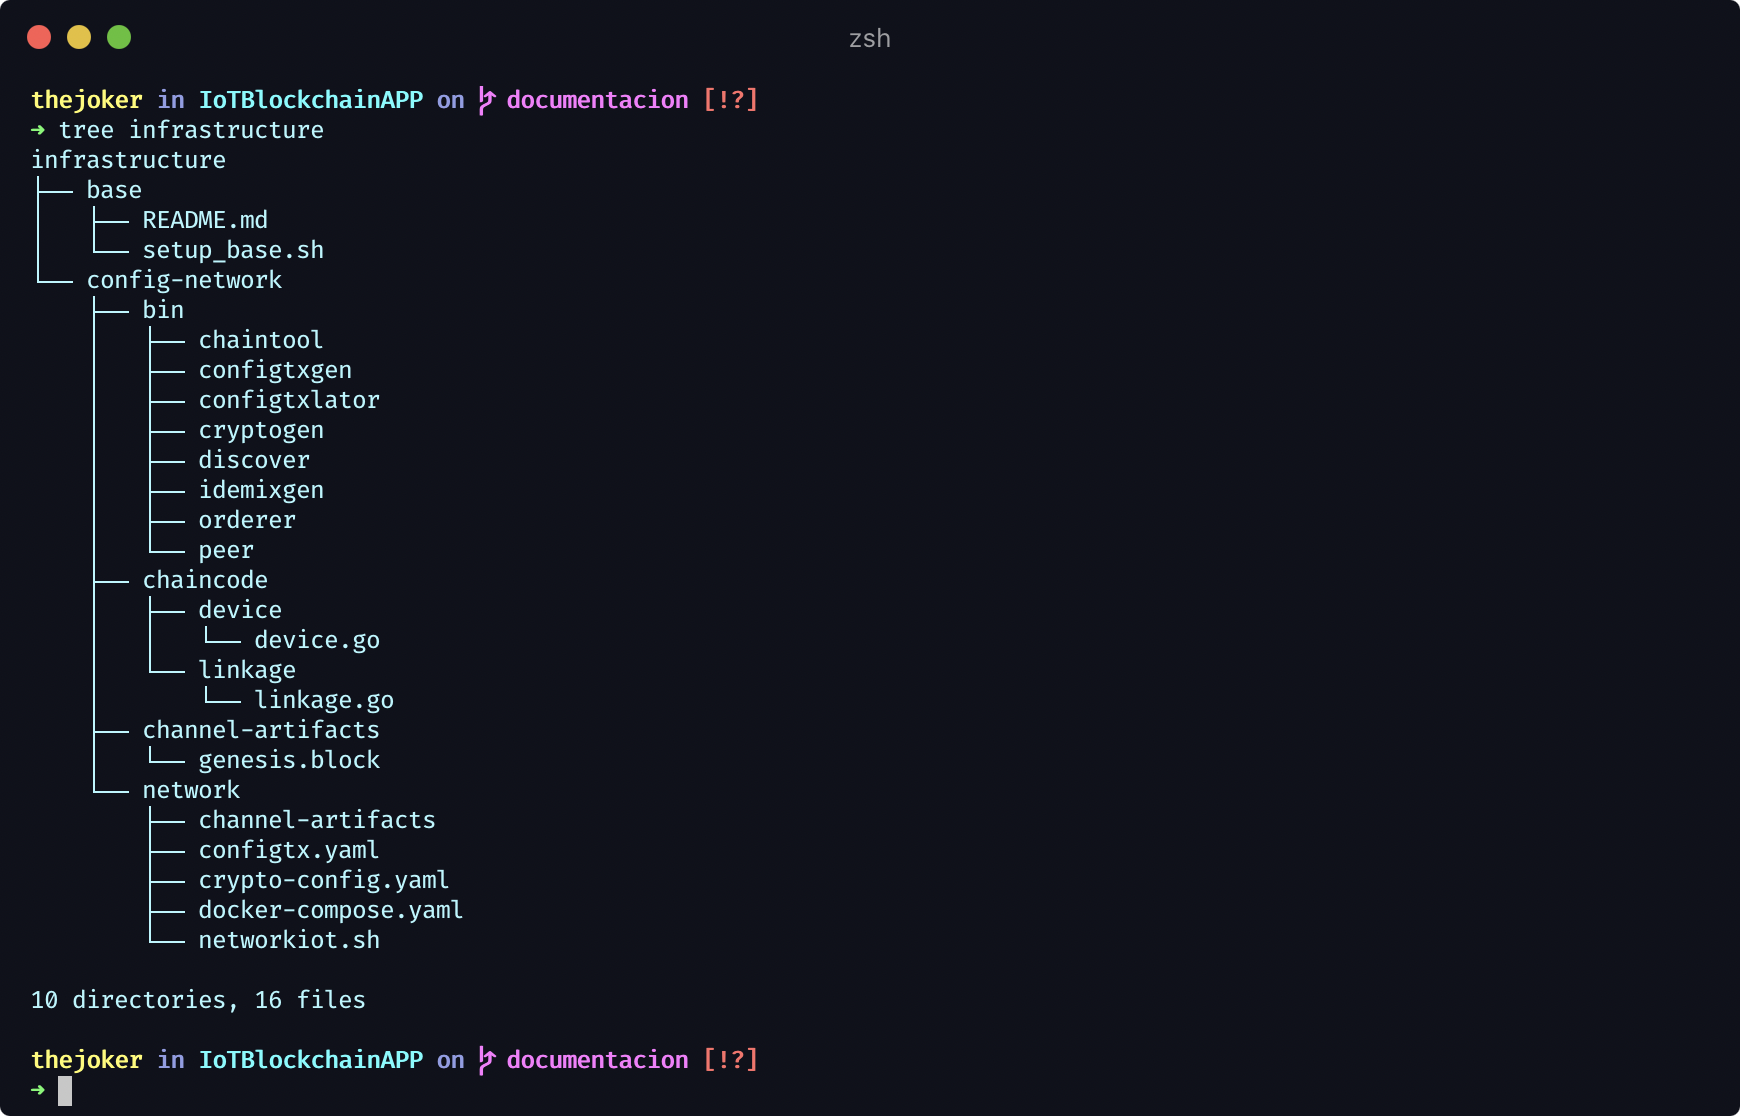
\includegraphics[width=10cm]{imagenes/desarrollo/tree_infraestructure}
  \caption{Tree de la carpeta infraestructure.}
  \label{fig:tree-infraestructure}
\end{figure}

\begin{figure}[ht!]
  \centering
  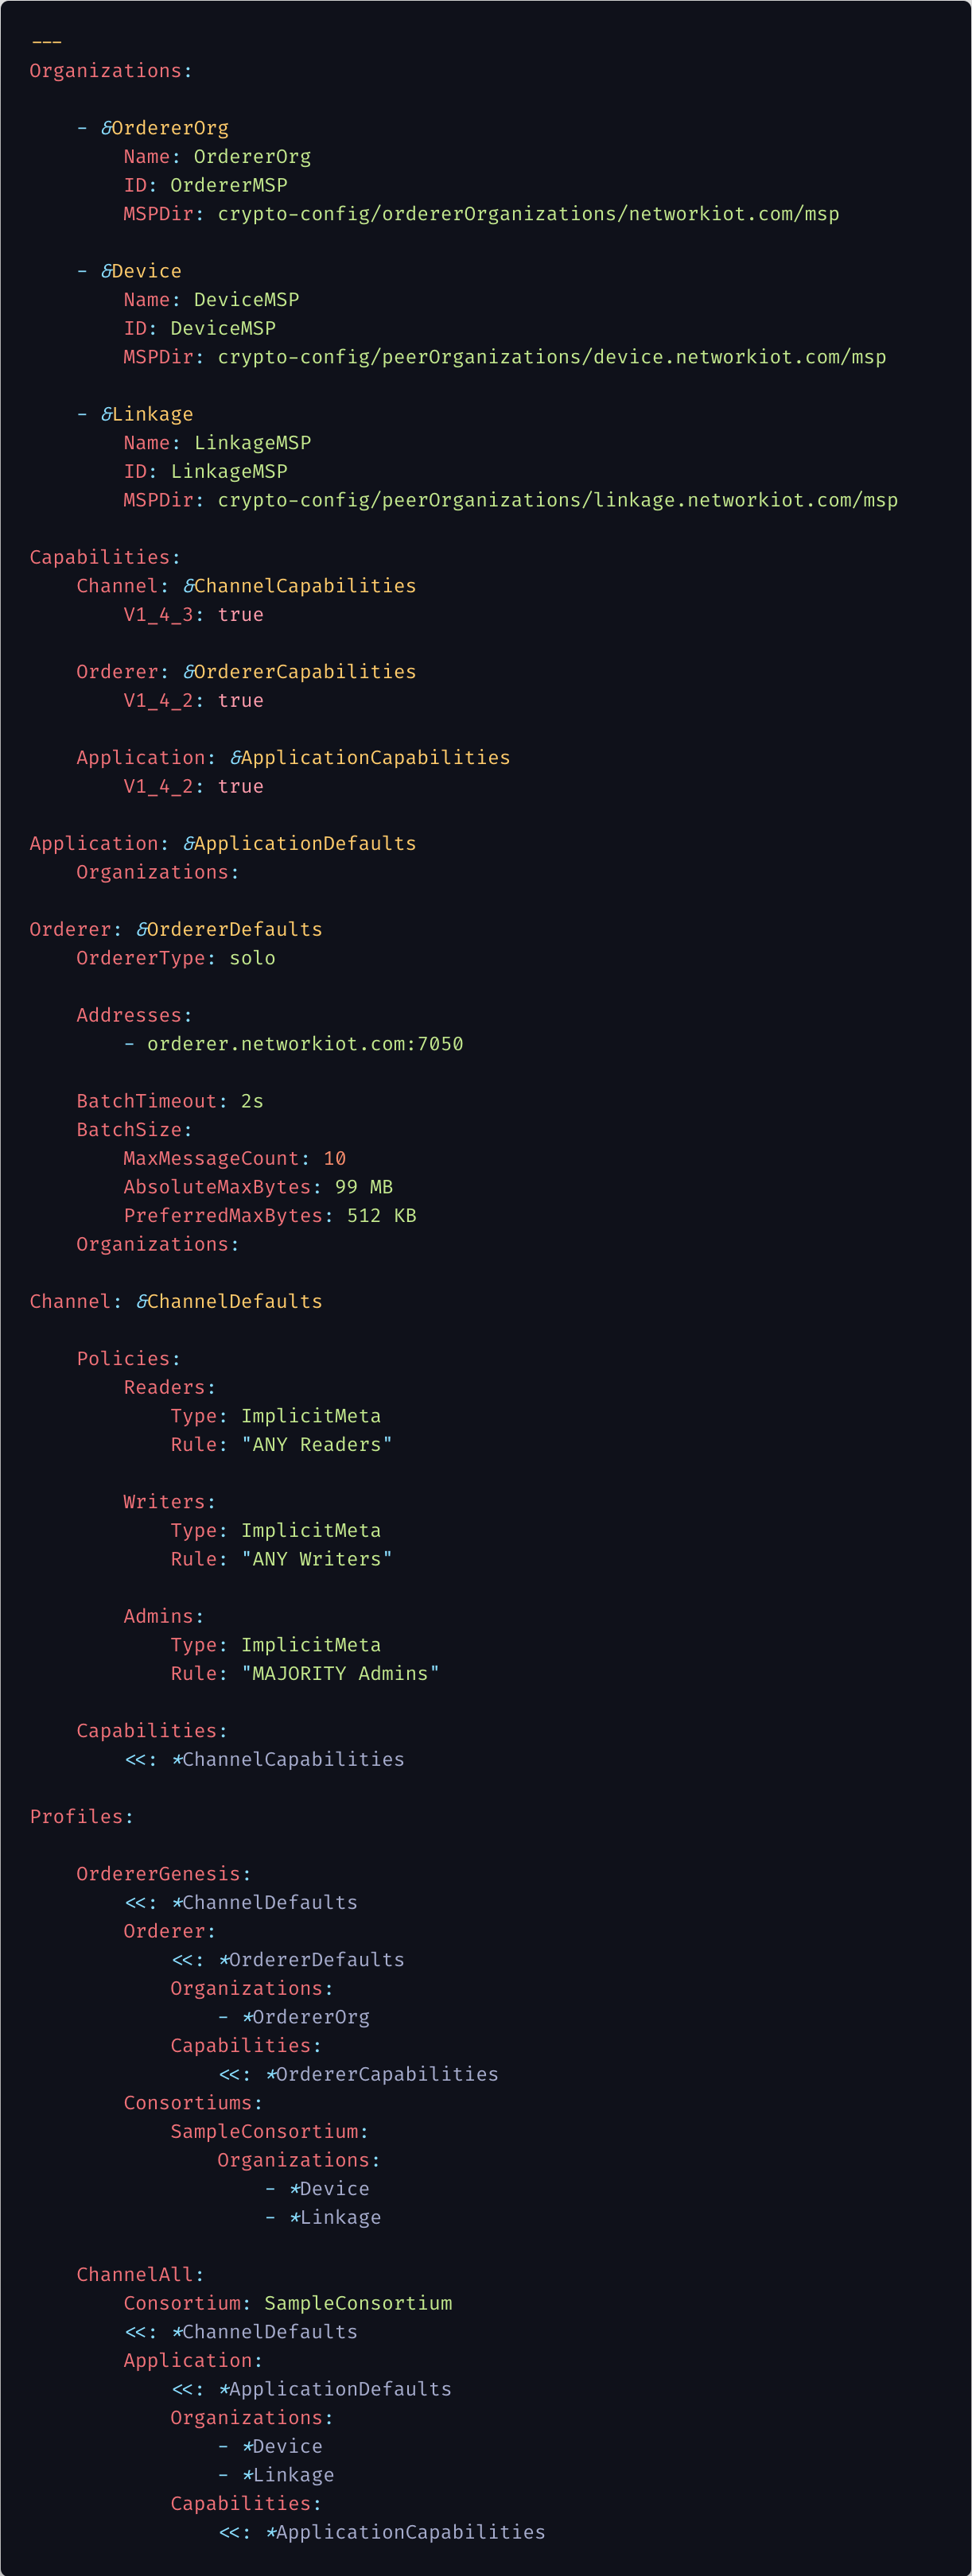
\includegraphics[width=10cm]{imagenes/desarrollo/configtx}
  \caption{Configtx de la red Blockchain.}
  \label{fig:configtx-blockchain}
\end{figure}

\begin{figure}[ht!]
  \centering
  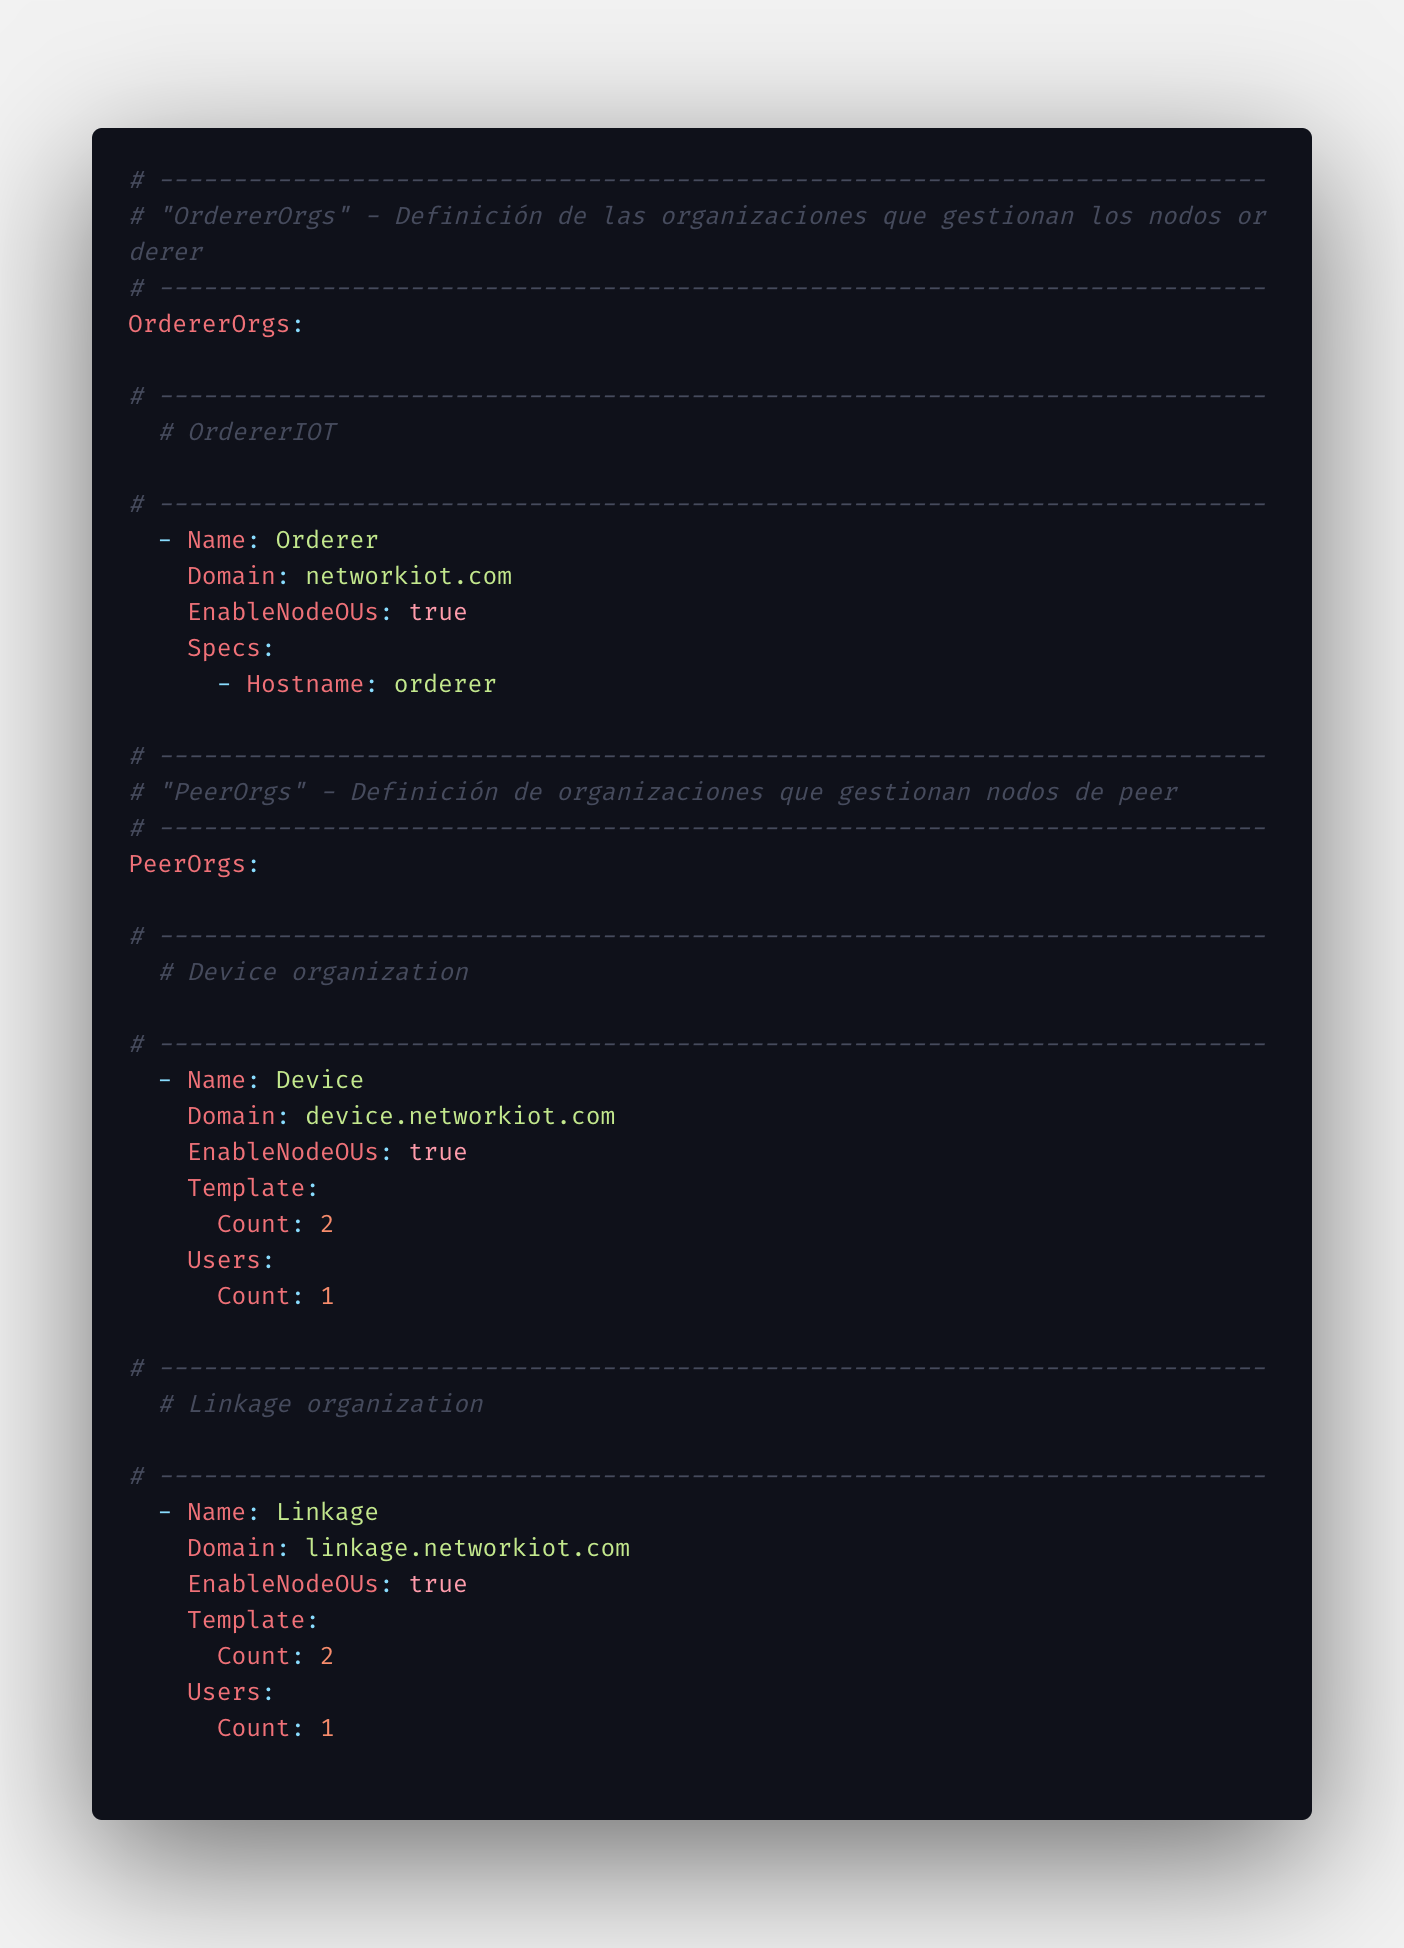
\includegraphics[width=10cm]{imagenes/desarrollo/crypto-config}
  \caption{Crypto-config de la red Blockchain.}
  \label{fig:crypto-config-blockchain}
\end{figure}

\subsubsection{Arquitectura de la red Blockchain.}

\begin{figure}[ht!]
  \centering
  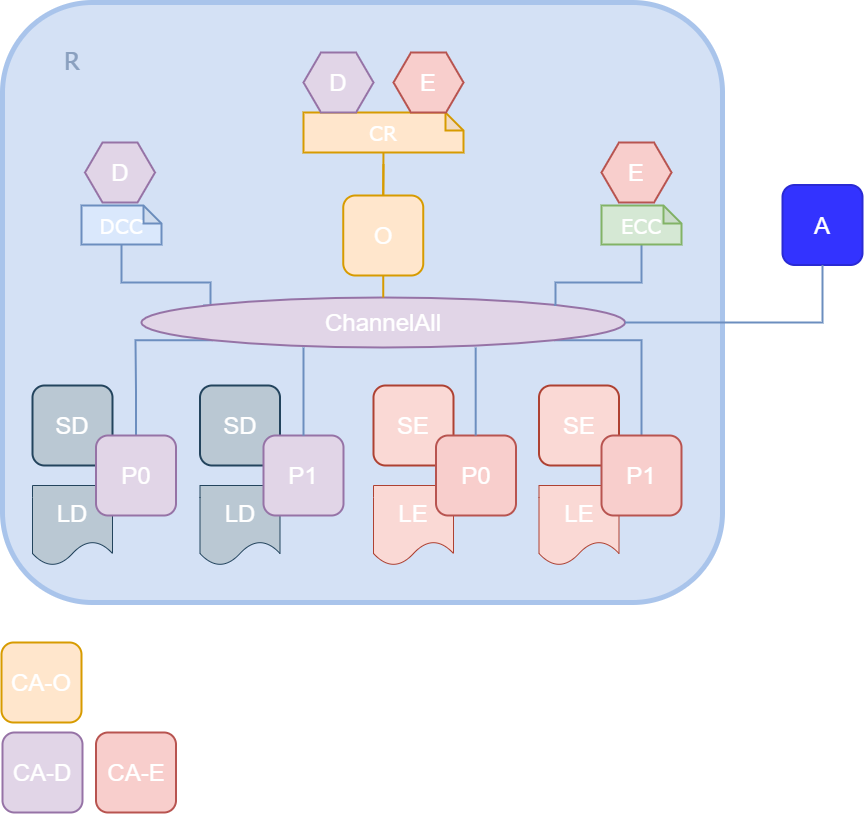
\includegraphics[width=10cm]{imagenes/desarrollo/arquitectura_networkiot}
  \caption{Arquitectura de la red Blockchain.}
  \label{fig:arquitectura-blockchain}
\end{figure}

\begin{figure}[ht!]
  \centering
  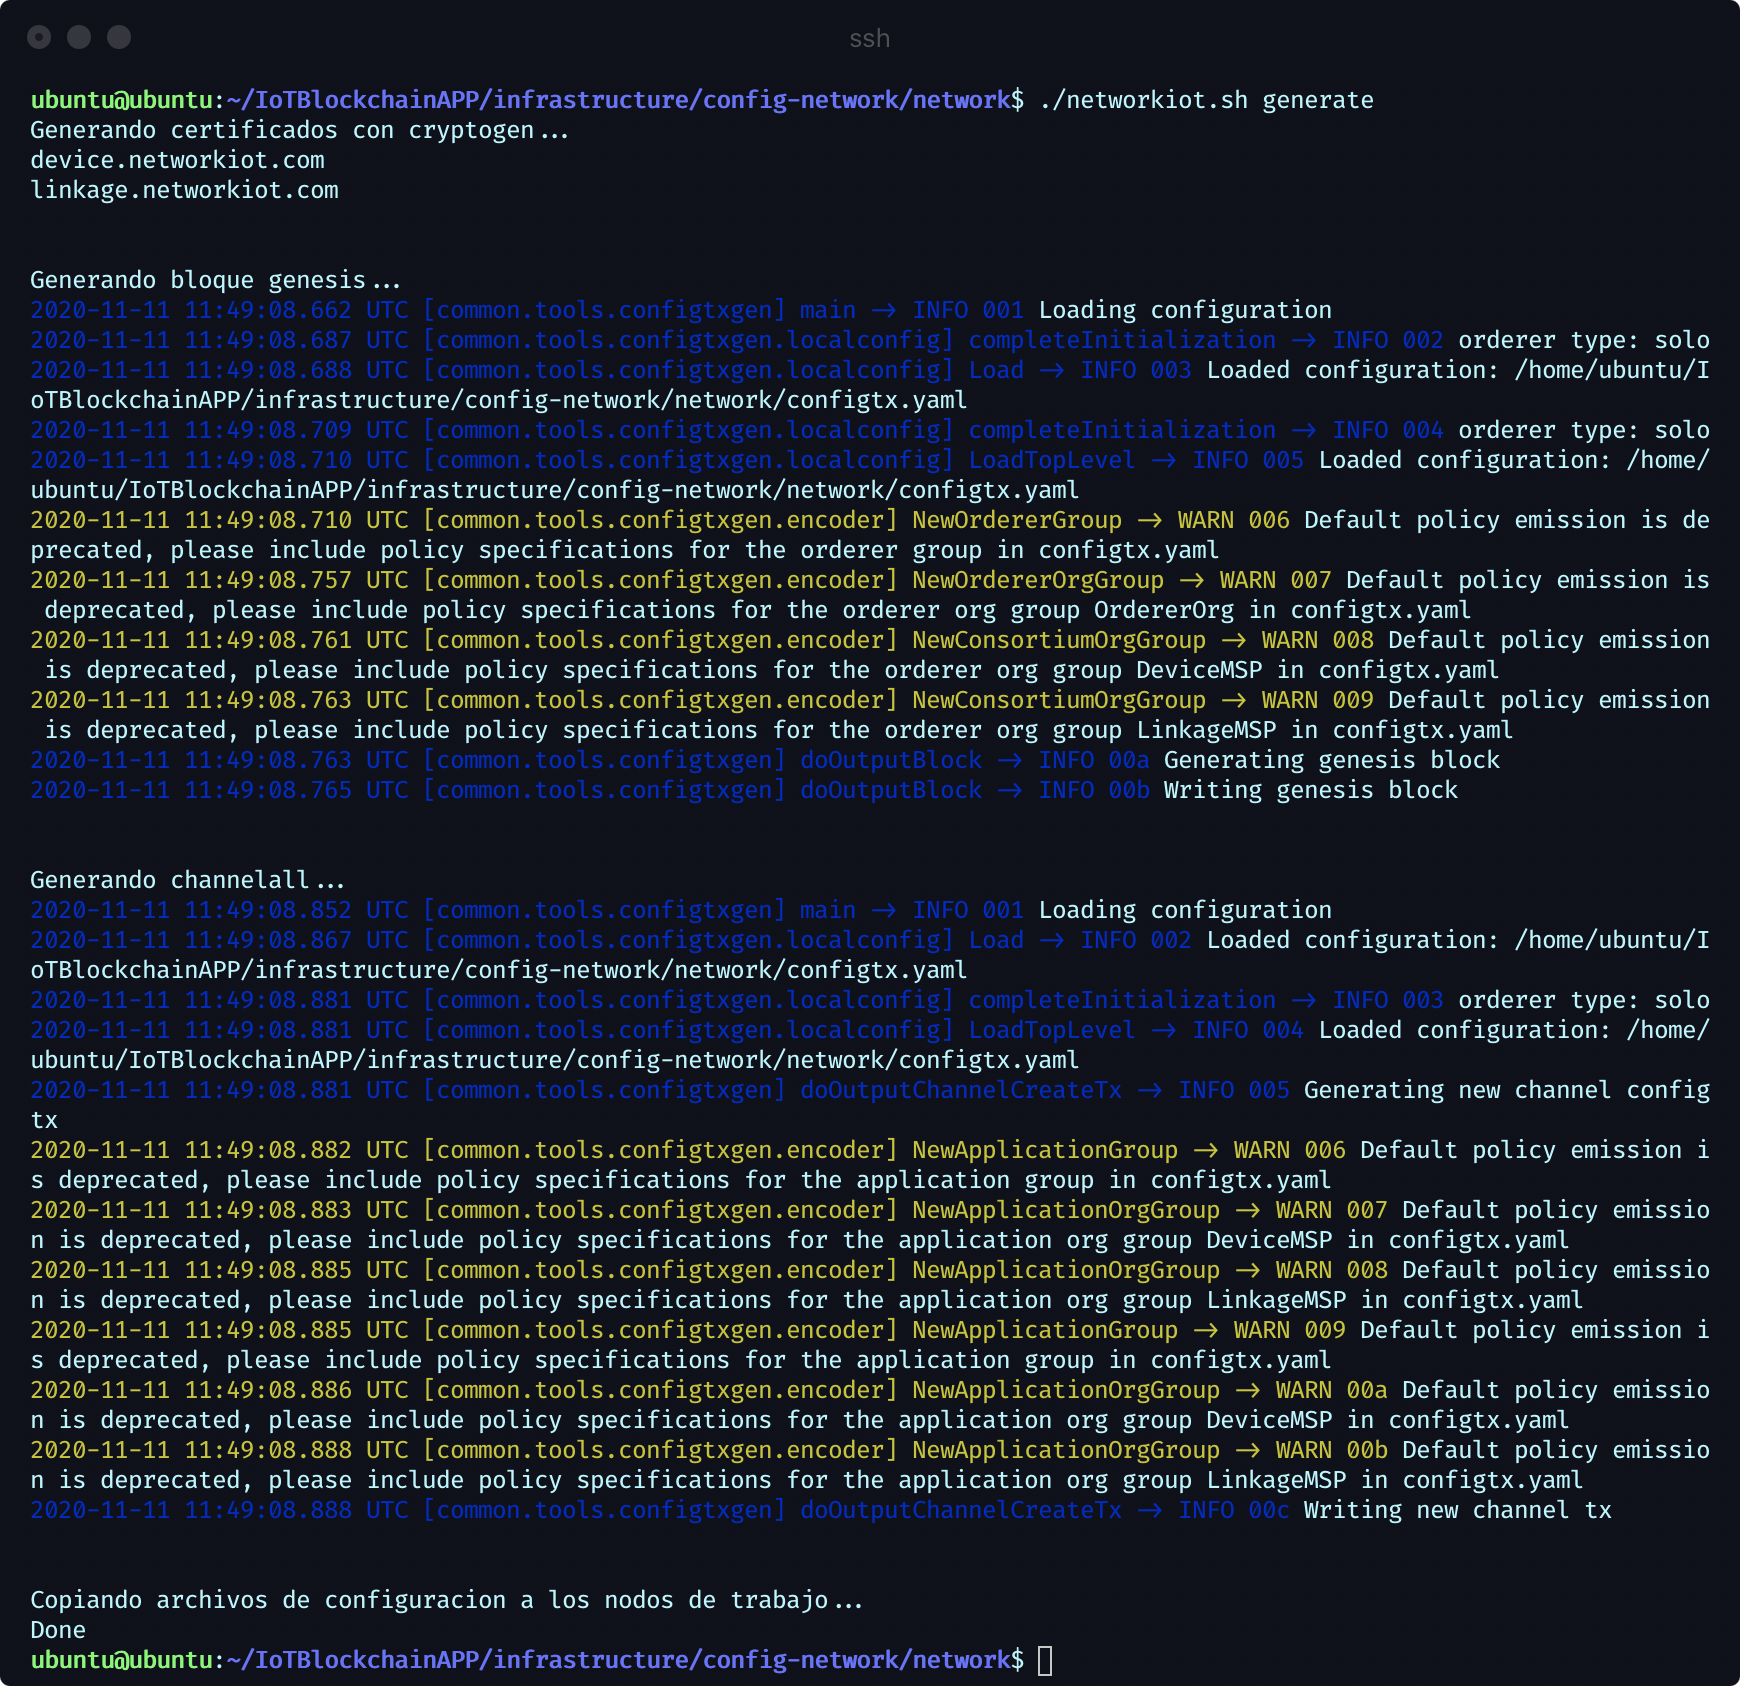
\includegraphics[width=10cm]{imagenes/desarrollo/comandos/generate}
  \caption{Opción generate del script networkiot.}
  \label{fig:generate}
\end{figure}

\begin{figure}[ht!]
  \centering
  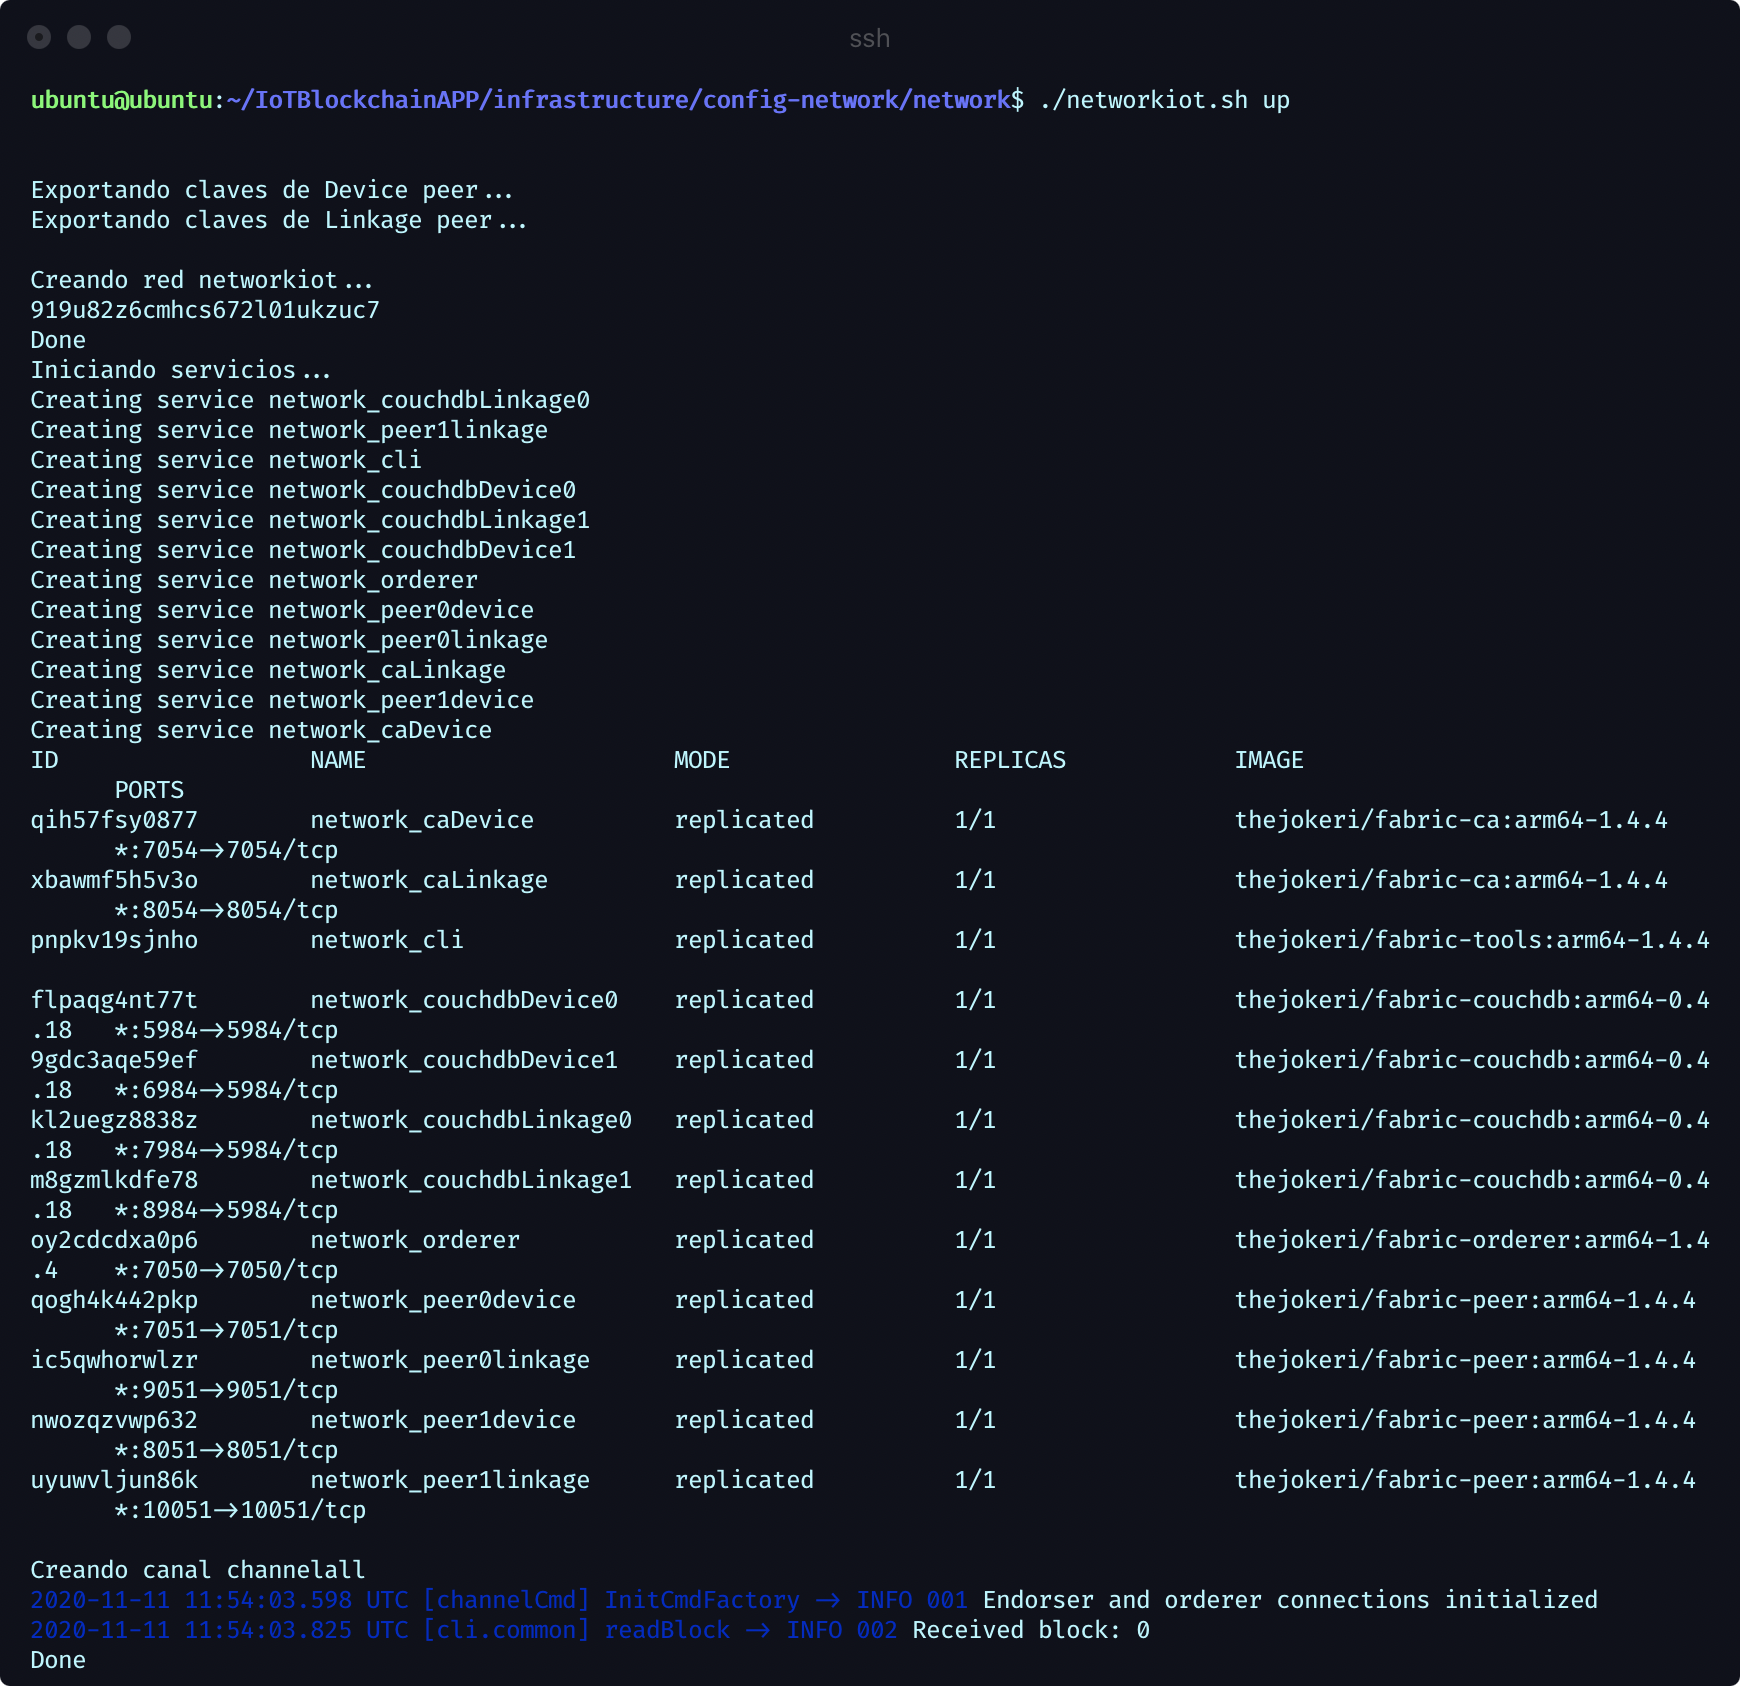
\includegraphics[width=10cm]{imagenes/desarrollo/comandos/up_1}
  \caption{Salida 1 de la opción up del script networkiot.}
  \label{fig:up-1}
\end{figure}

\begin{figure}[ht!]
  \centering
  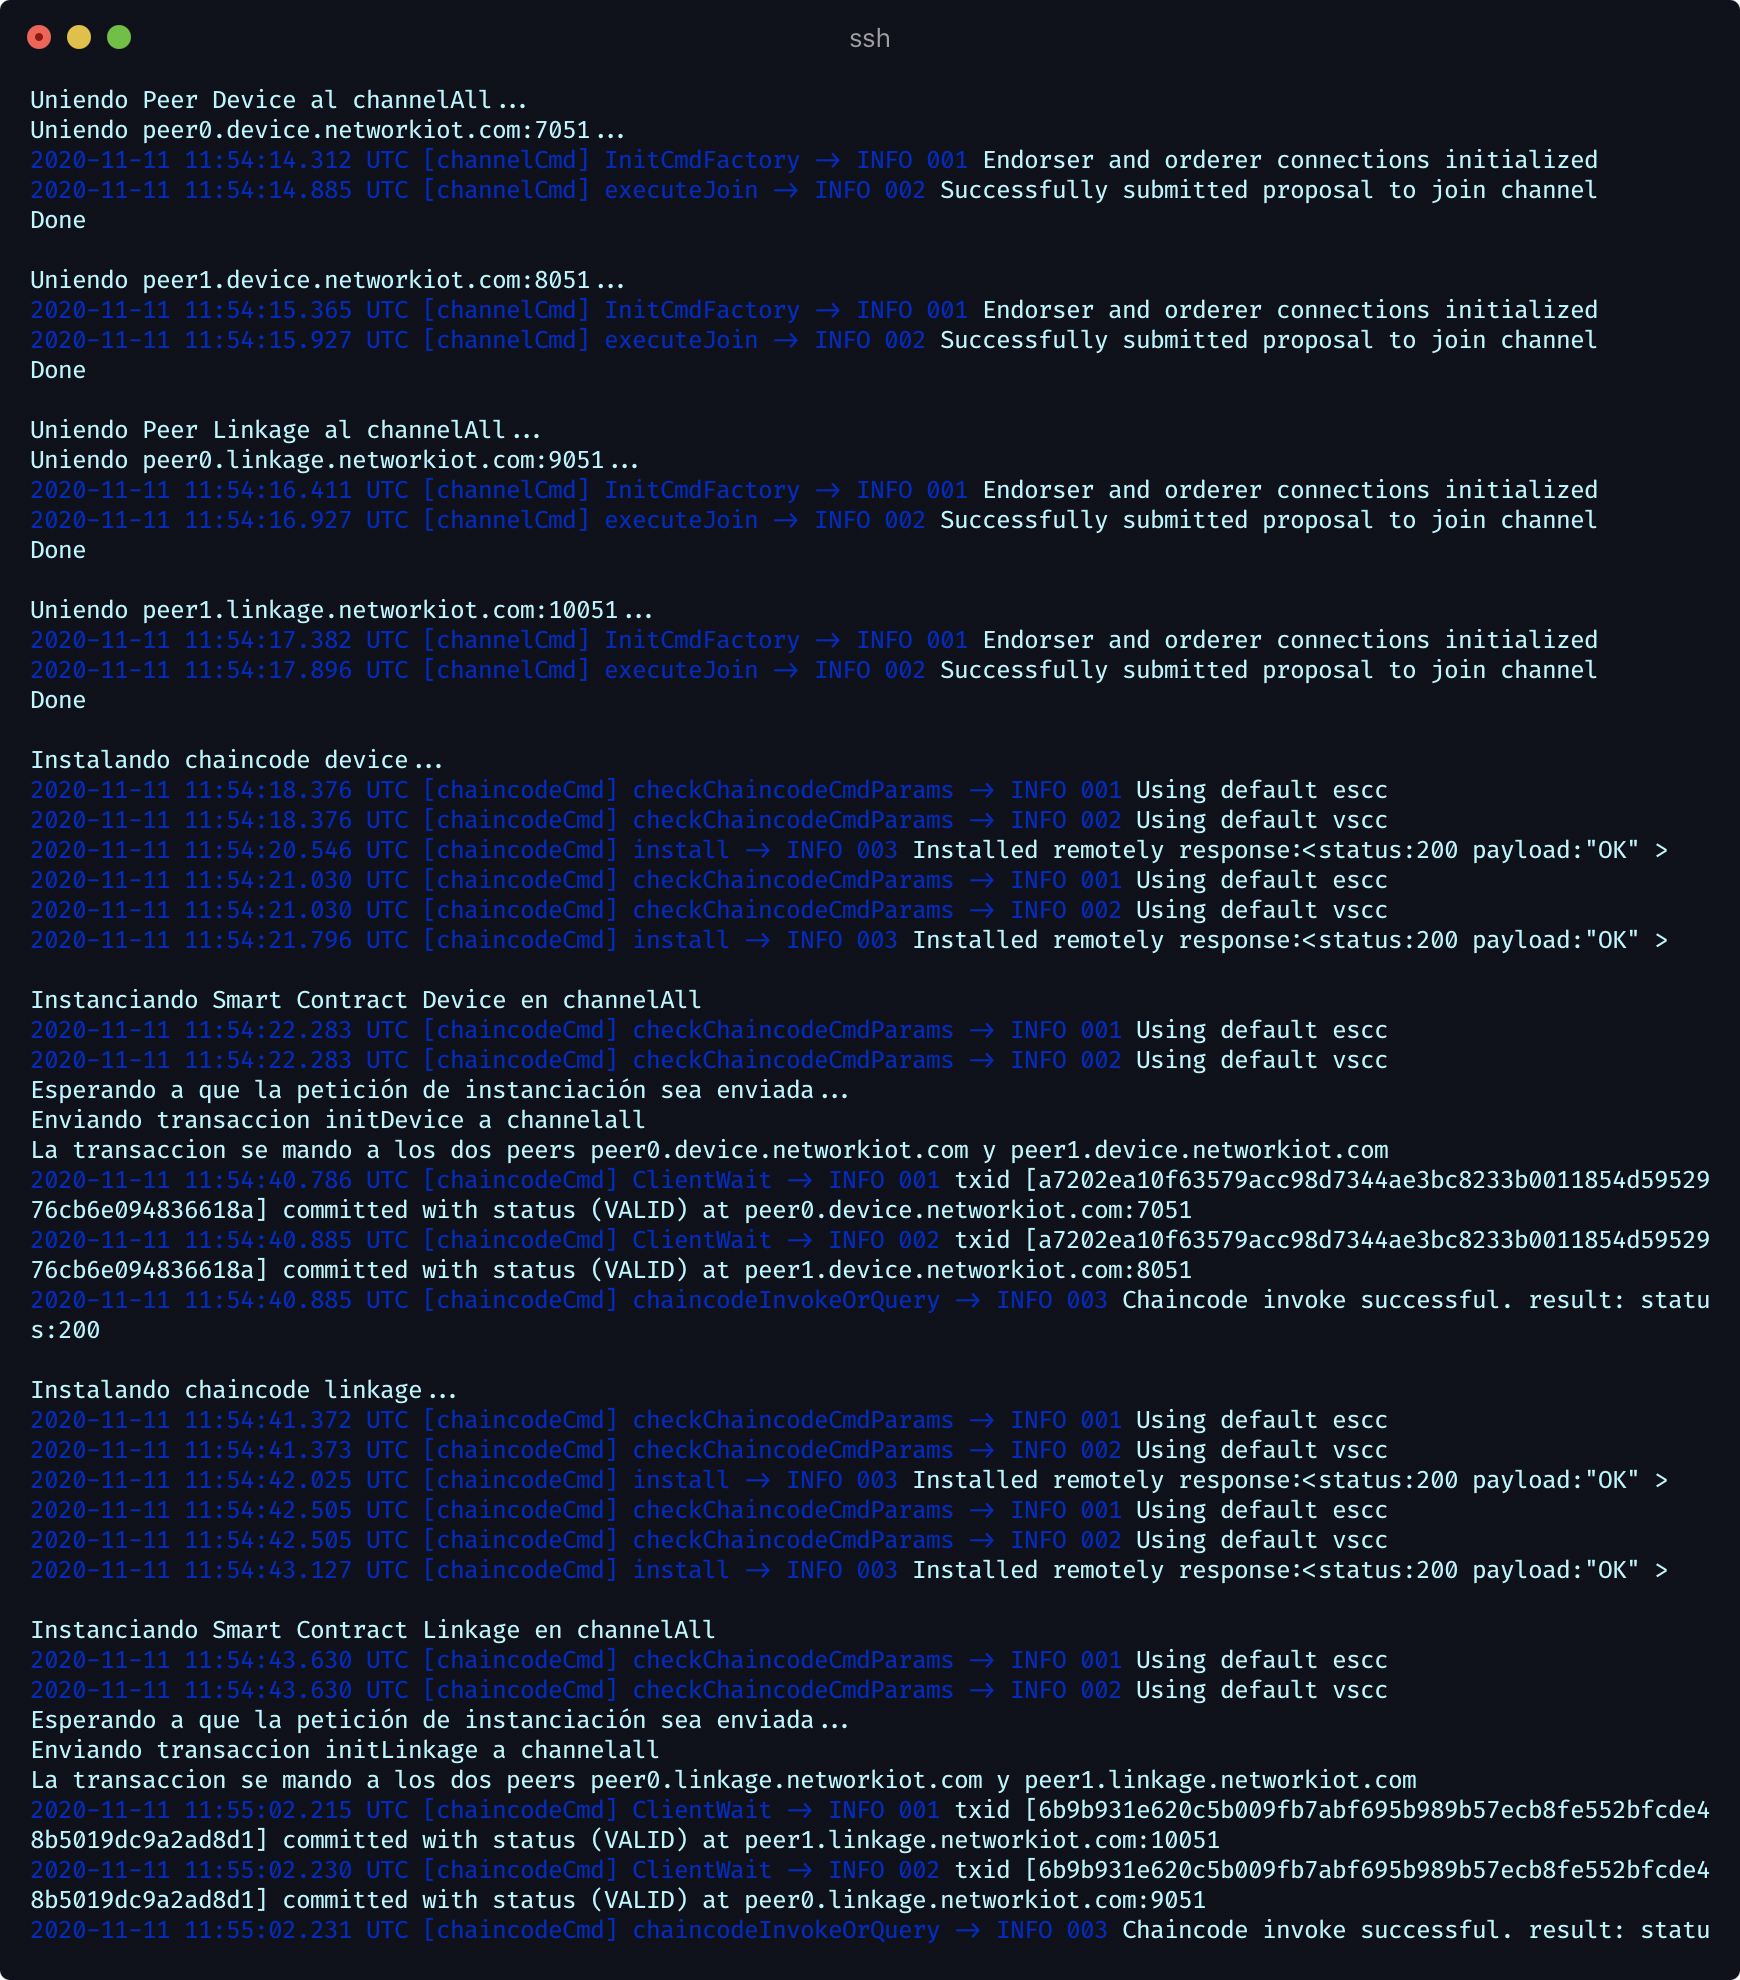
\includegraphics[width=10cm]{imagenes/desarrollo/comandos/up_2}
  \caption{Salida 2 de la opción up del script networkiot.}
  \label{fig:up-2}
\end{figure}

\begin{figure}[ht!]
  \centering
  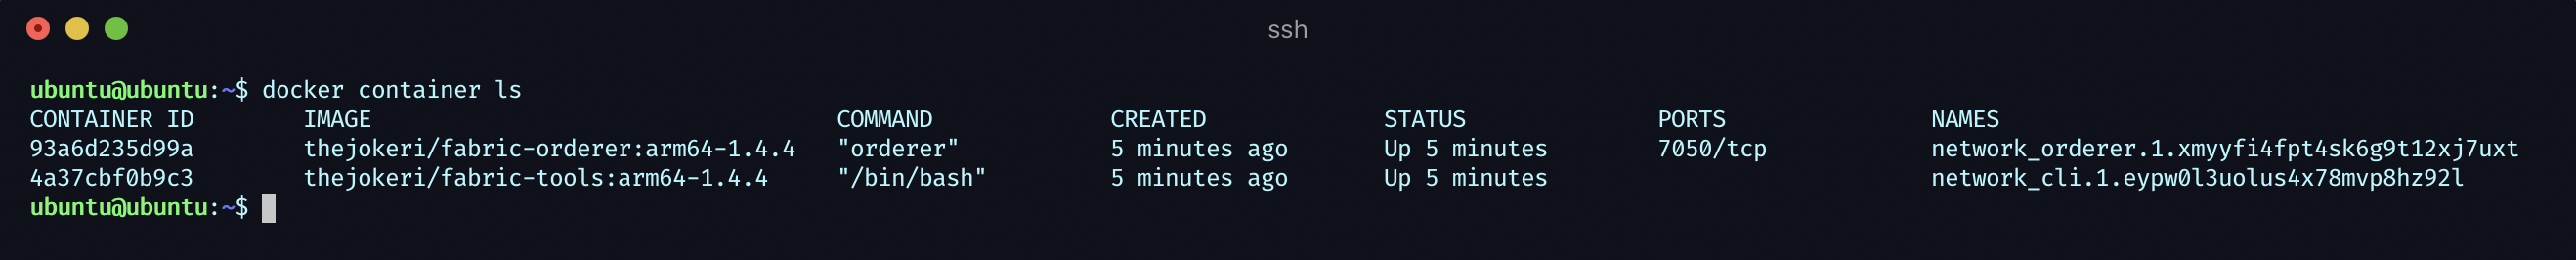
\includegraphics[width=10cm]{imagenes/desarrollo/comandos/containers_master}
  \caption{Salida de contenedores en el nodo maestro.}
  \label{fig:containers-master}
\end{figure}

\begin{figure}[ht!]
  \centering
  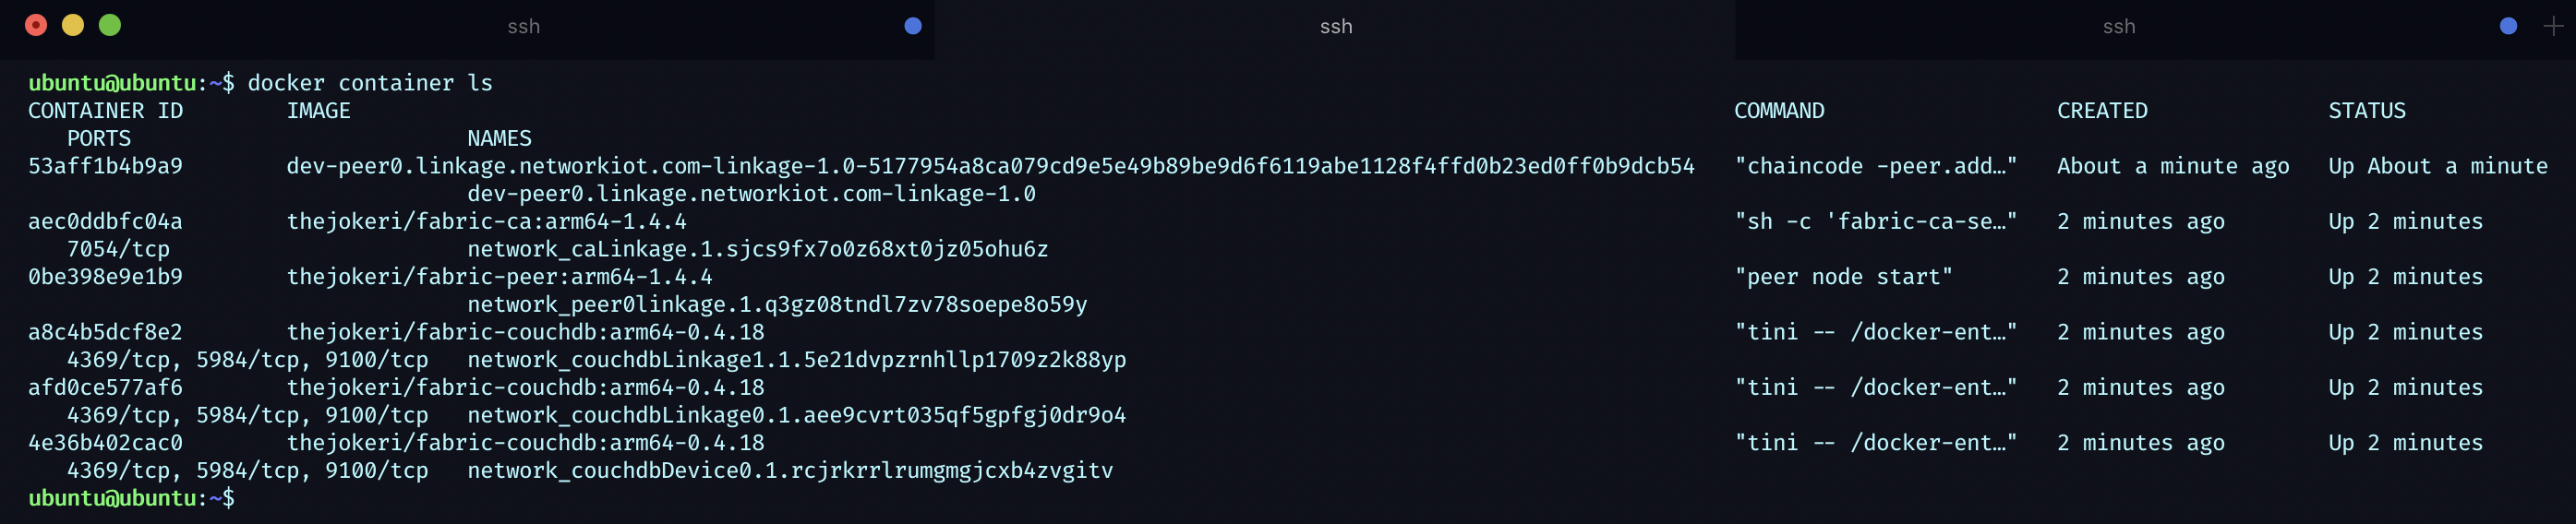
\includegraphics[width=10cm]{imagenes/desarrollo/comandos/containers_worker1}
  \caption{Salida de contenedores en el nodo worker 1.}
  \label{fig:containers-worker1}
\end{figure}

\begin{figure}[ht!]
  \centering
  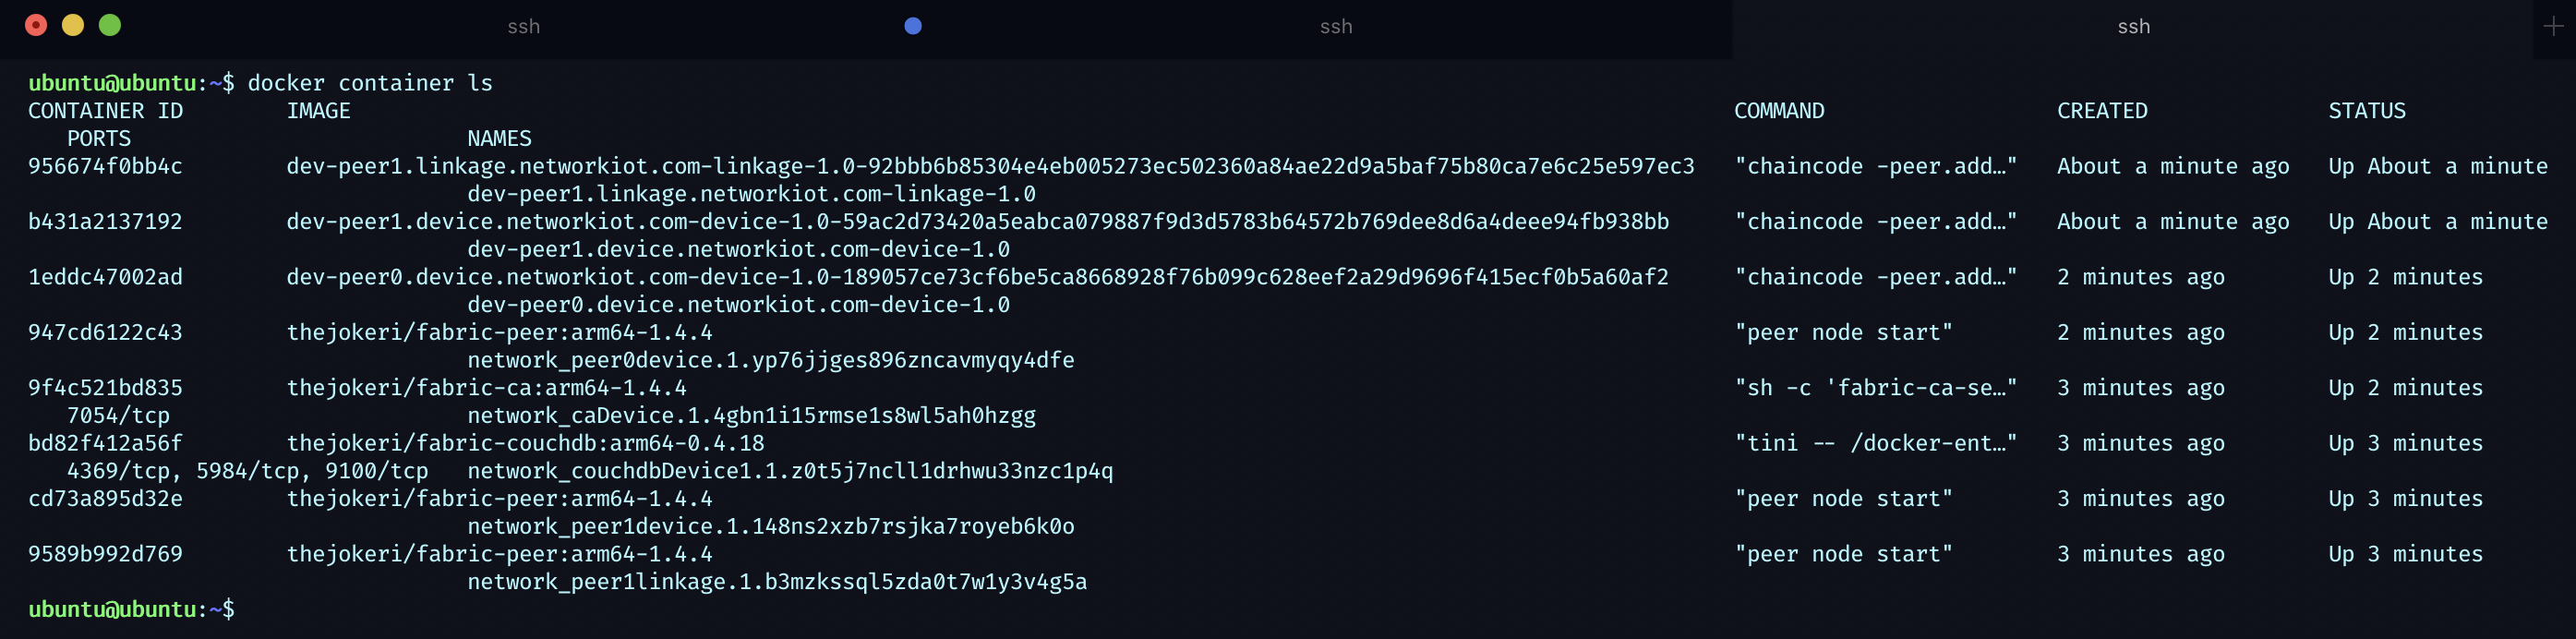
\includegraphics[width=10cm]{imagenes/desarrollo/comandos/containers_worker2}
  \caption{Salida de contenedores en el nodo worker 2.}
  \label{fig:containers-worker2}
\end{figure}

\begin{figure}[ht!]
  \centering
  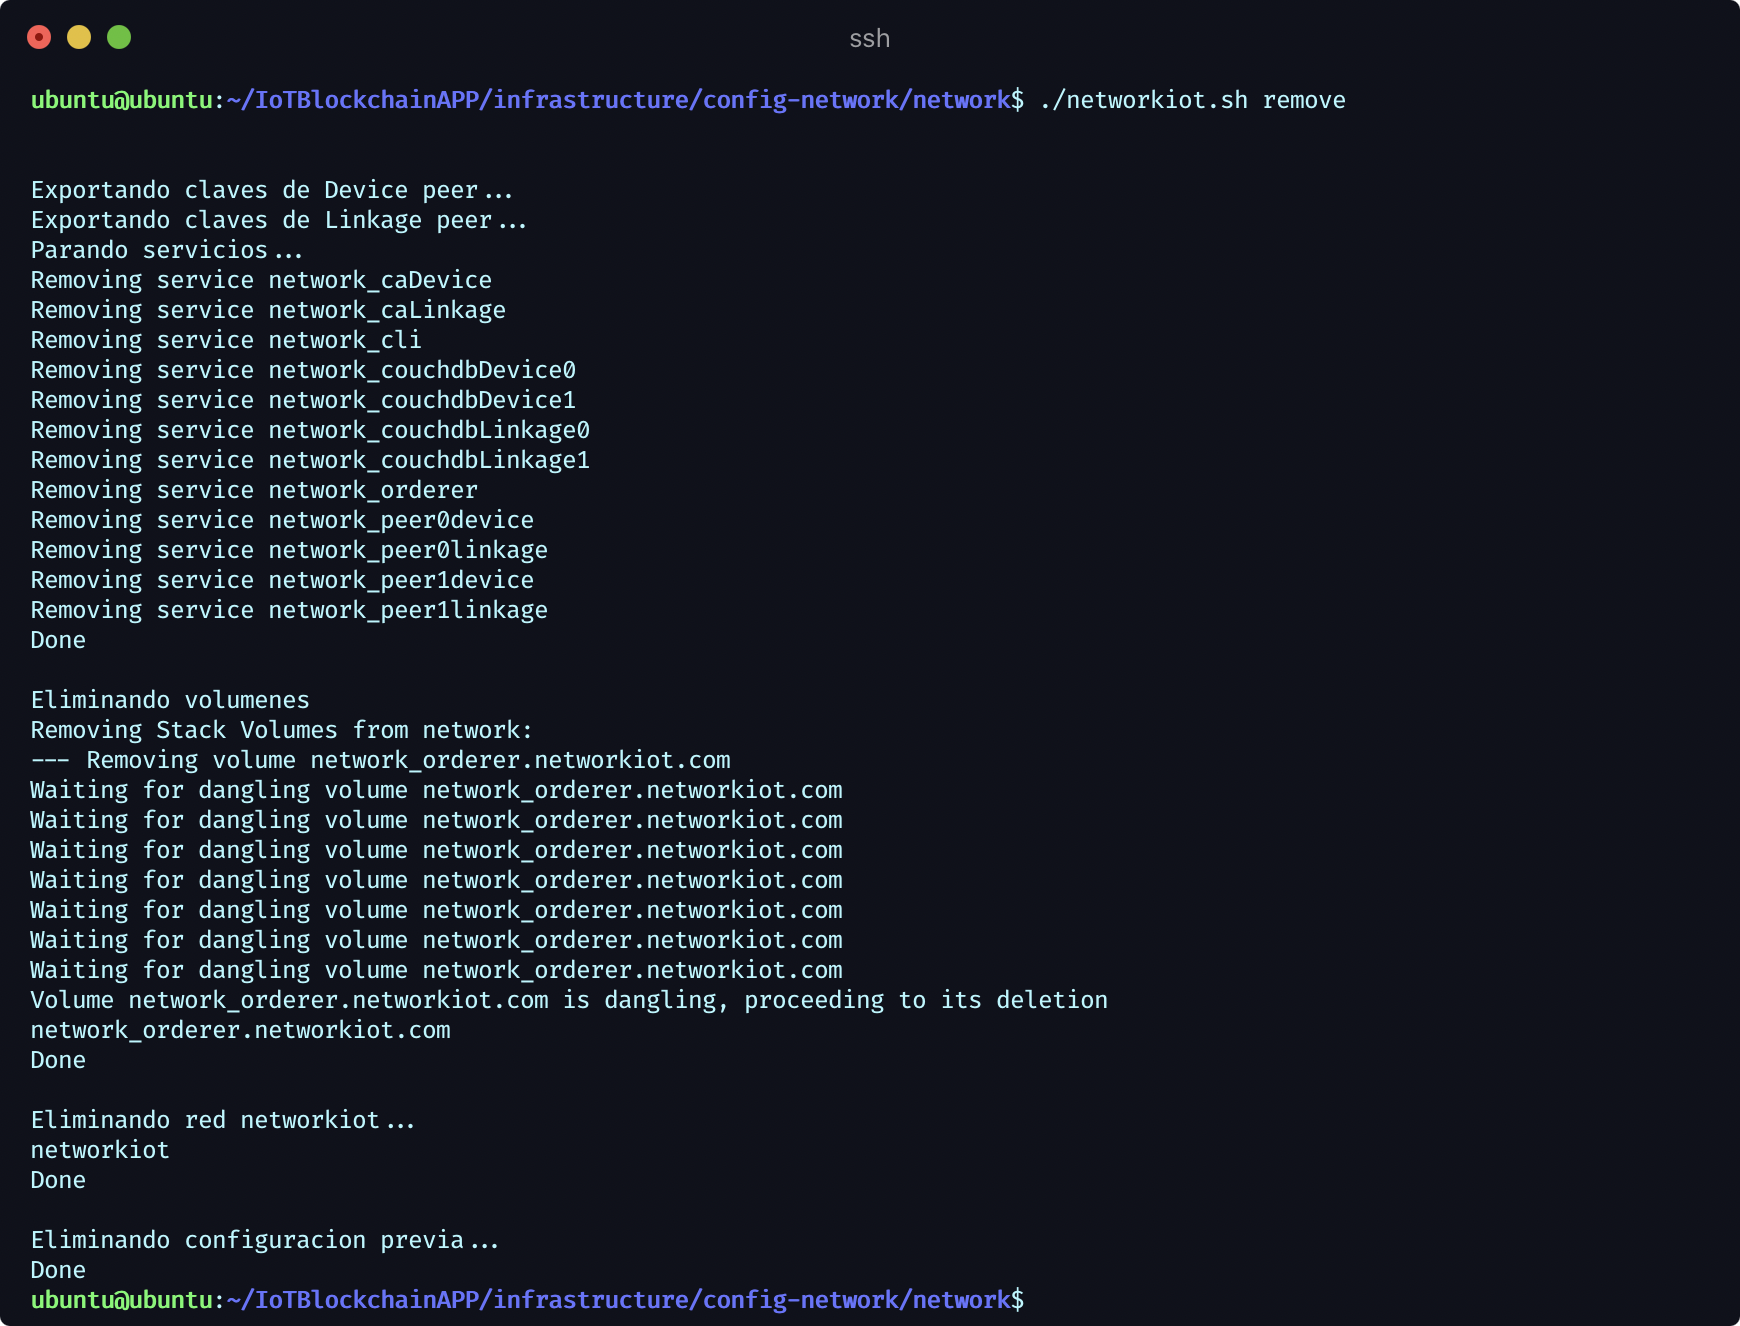
\includegraphics[width=10cm]{imagenes/desarrollo/comandos/remove}
  \caption{Opción remove del script networkiot.}
  \label{fig:remove}
\end{figure}

\subsection{Desarrollo del Back end.}

\begin{figure}[ht!]
  \centering
  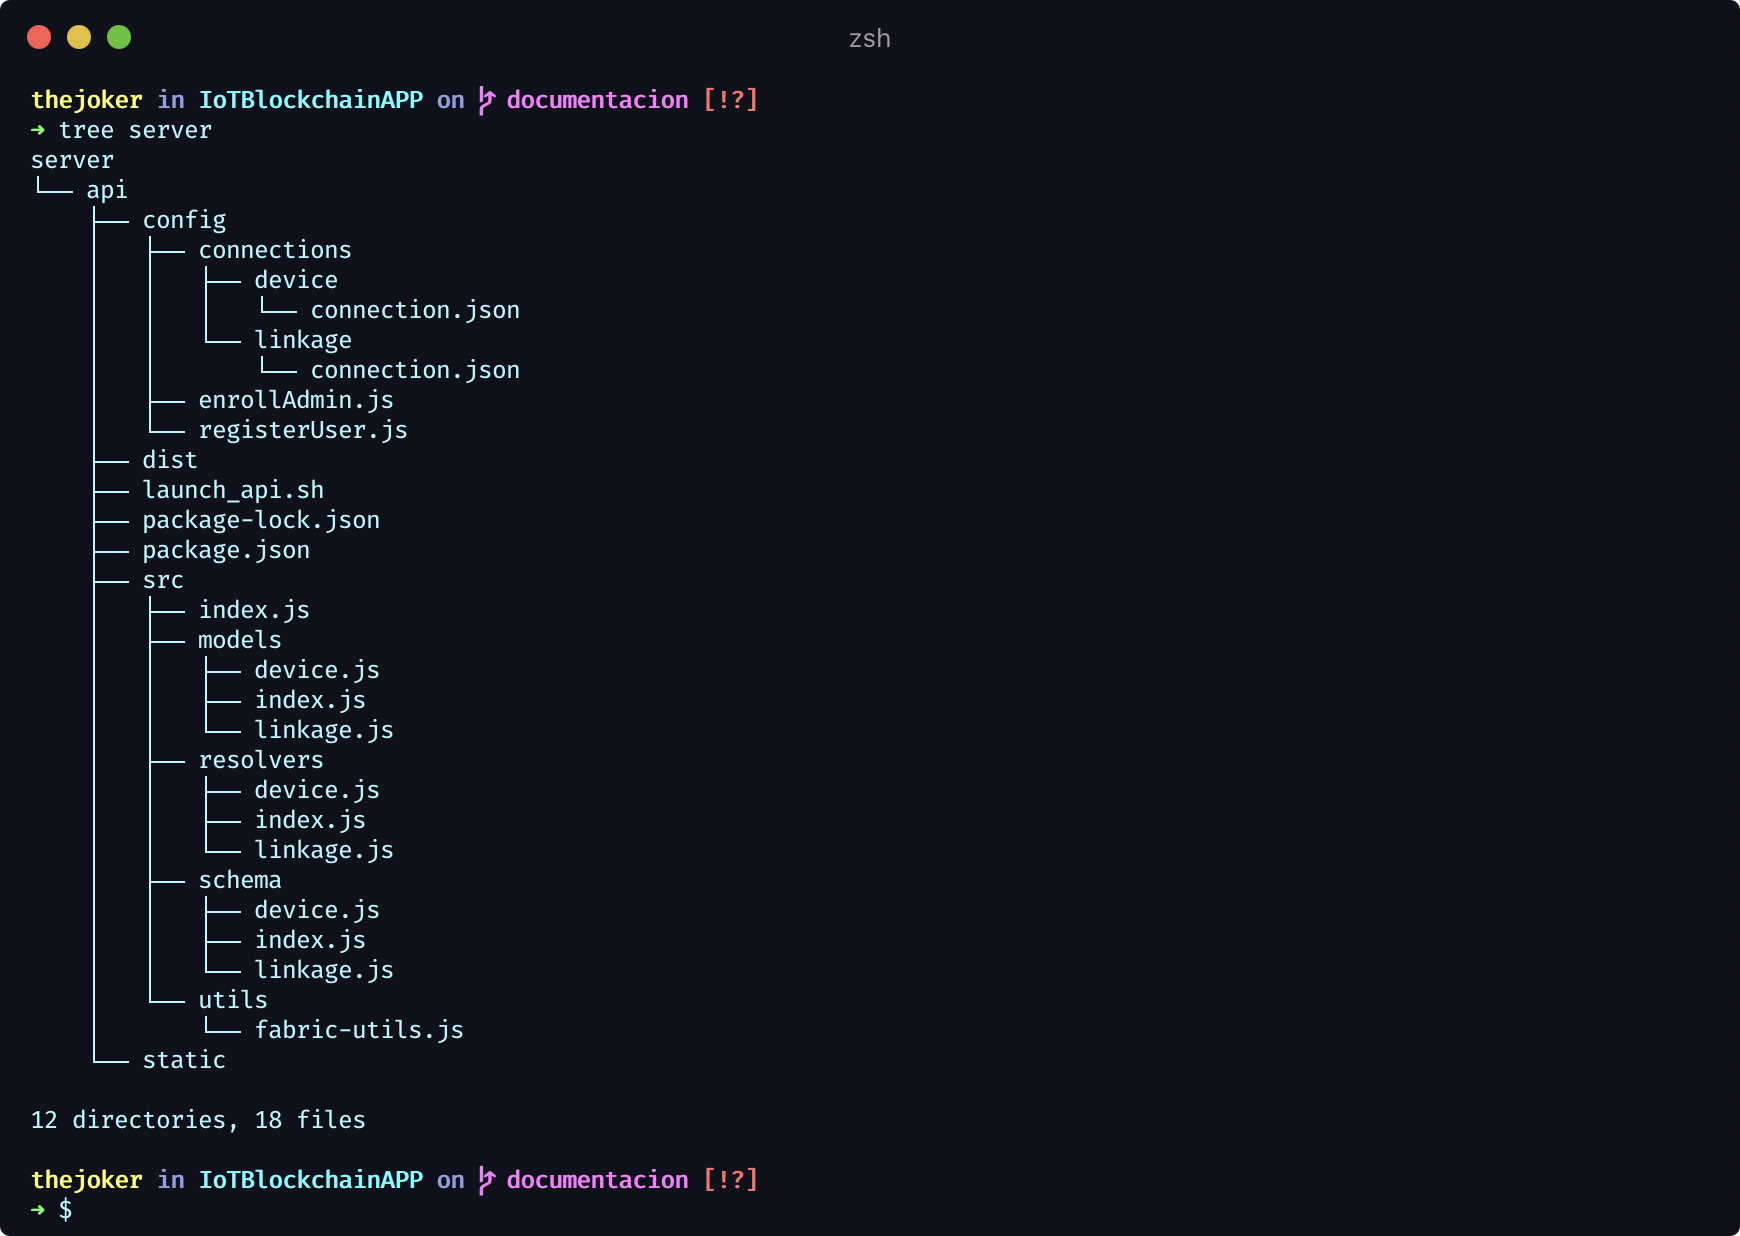
\includegraphics[width=10cm]{imagenes/desarrollo/tree_server}
  \caption{Tree de la carpeta server.}
  \label{fig:tree-server}
\end{figure}

\begin{figure}[ht!]
  \centering
  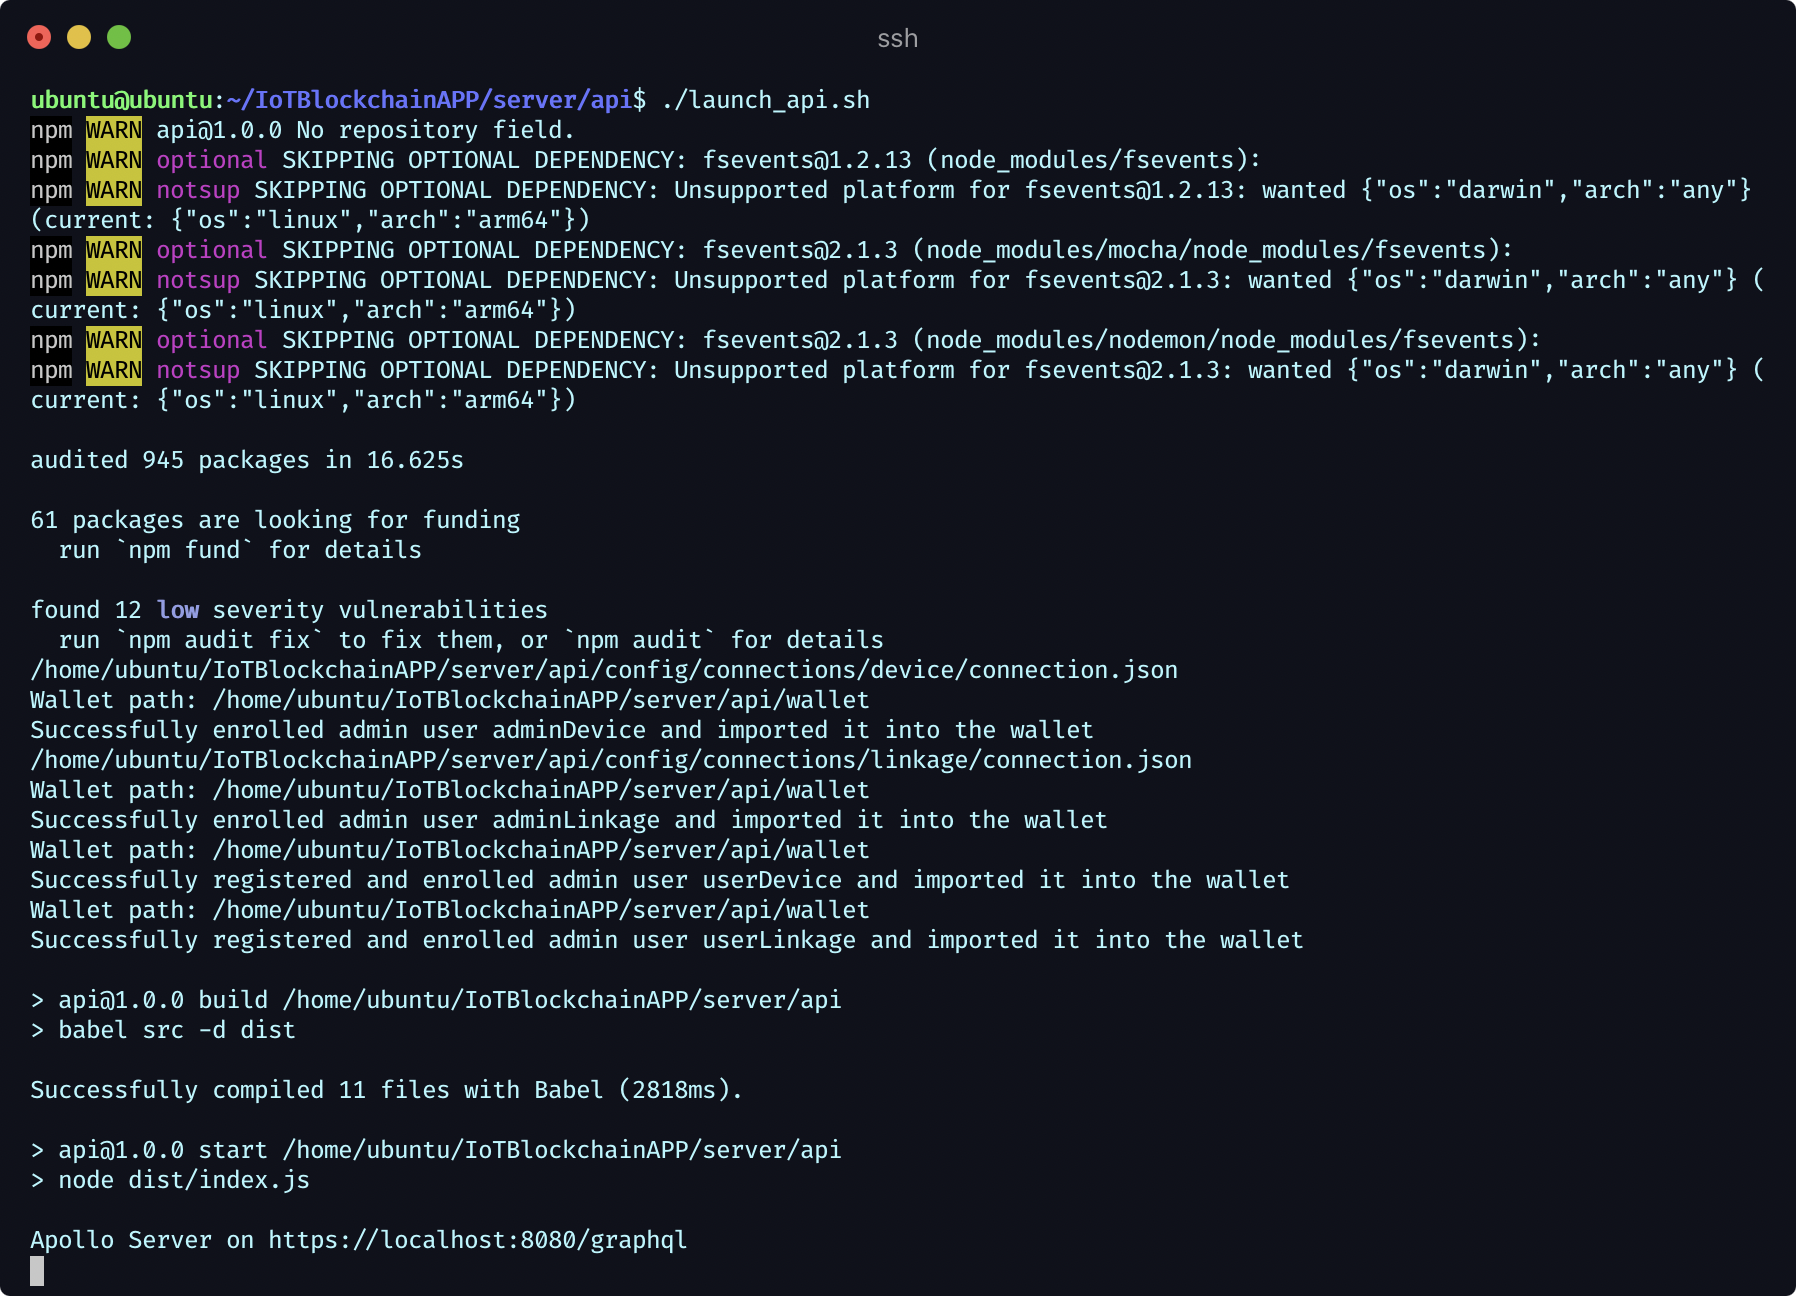
\includegraphics[width=10cm]{imagenes/desarrollo/comandos/launch_api}
  \caption{Ejecución del script launch\_api.}
  \label{fig:launch-api}
\end{figure}

\subsection{Desarrollo del Front end y despliegue.}

\begin{figure}[ht!]
  \centering
  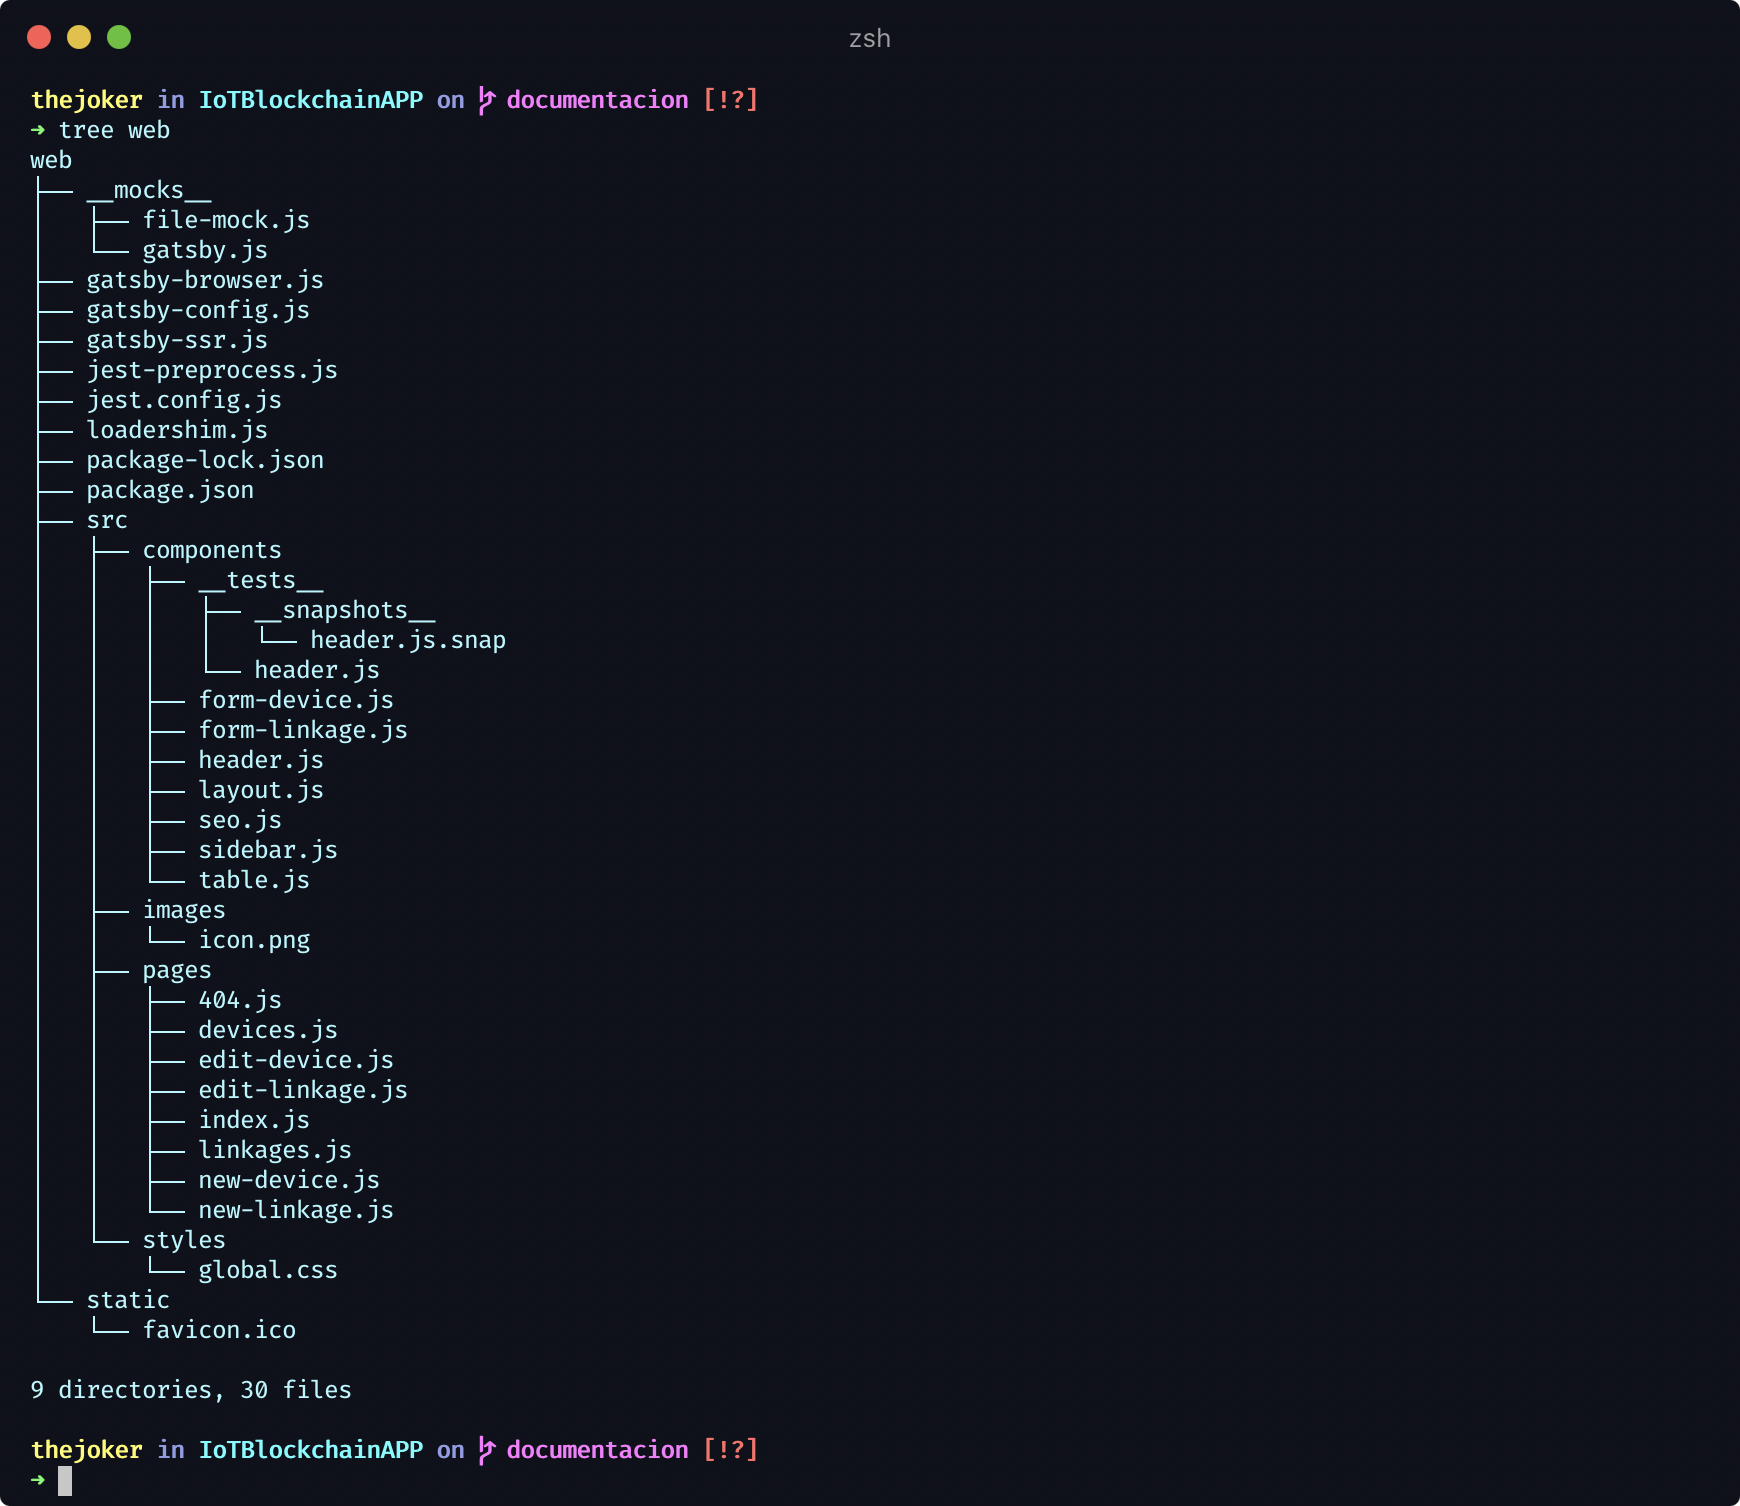
\includegraphics[width=10cm]{imagenes/desarrollo/tree_web}
  \caption{Tree de la carpeta web.}
  \label{fig:tree-web}
\end{figure}

\subsection{Conclusión.}

\newpage